% =====================================================================
%  c18 —— 原文印刷页 149–155（PDF 第 150–156 页）
%  含：5.1.1（三级标题）、5.2（二级标题）、5.2.1（三级标题）；
%  插图 Fig. 23–27；编号公式 (5.6)–(5.23)。
%  说明：本片段不含 \section 级标题（原文「5.2」为二级标题，按编号点数
%  对应 \subsection），故按规范不插入 keytakeaways。
% =====================================================================

而 $X'$ 是另一条从 $Y'$ 到 $Y''$ 的有向配边（bordism）
\begin{equation*}
  (\partial X')_{\mathrm{in}}=Y' \qquad (\partial X)_{\mathrm{out}}=Y''
\end{equation*}
那么我们便可如 {\small\itshape ［原文标记：(??)］} 那样作复合 $X'\circ X$，得到从 $Y$ 到 $Y''$ 的配边。
% [原文待办标记，原文 p.149：交叉引用未解析，页面显示为 (??)，所指应为附录 L 或正文前文中配边复合的定义式]
% [Tutor Note: 原文此处的两个边界条件写成 $(\partial X')_{\mathrm{in}}=Y'$ 与 $(\partial X)_{\mathrm{out}}=Y''$，第二式漏了撇号；按文意（$X'$ 是从 $Y'$ 到 $Y''$ 的配边）它应是 $(\partial X')_{\mathrm{out}}=Y''$。译文照原文转写、未擅自订正；对照第 148 页关于 $X:Y\to Y'$ 的边界约定即可确认这是笔误]

再自然不过的是，我们希望相应的线性映射也复合起来：
\begin{equation*}
  F(X'\circ X)=F(X')\circ F(X):\mathcal{H}(Y)\to\mathcal{H}(Y'')
\end{equation*}

我们所描述的，用数学术语说，就是范畴之间的一个函子（functor）。关于范畴的背景材料见附录 K。在描述了上述框架的若干变体之后，我们将更详细地解释这幅范畴论的图景。

\subsubsection{更多的结构} % 原文: 5.1.1 More Structure

我们可以把上述图景看作一个基本框架：通过充实与空间 $X$、$Y$ 相伴的拓扑数据与几何数据，就能在这个框架上造出更有趣的理论。

例如，我们或许能够给 $X$ 与 $Y$ 赋予

\begin{enumerate}
  \item 定向、spin、spin$^c$、pin 结构等（对某些 $X$ 与 $Y$）；
  \item 复结构、共形结构、因果结构、Riemann 结构；
  \item 其他的场——带联络的主 $G$-丛、相伴丛的截面等。
\end{enumerate}

动机性的例子之一是二维共形场论。在那一情形，Segal 的公理建立在赋有共形结构的二维配边之上。

在考虑非拓扑理论时，会出现两个重要的复杂之处：

\begin{enumerate}
  \item 标度（scale）与重整化的概念变得重要。
  \item Hilbert 空间其实并不是对某个 $(d-1)$ 维流形定义的，而是对 $(d-1)$ 维流形周围 $d$-流形的一个芽（germ）定义的；于是算符代数还可以依赖于额外的结构，例如第二基本形式。{\small\itshape ［原文标记：此处应引 Segal 以为例］}
% [原文待办标记，原文 p.149：原文作 [CITE SEGAL for example]，作者留待补引 Segal 关于共形场论公理化的文献]
\end{enumerate}

\subsection{拓扑场论的定义} % 原文: 5.2 The Definition Of Topological Field Theory

关于配边理论的基本数学背景，见 {\small\itshape ［原文标记：附录 ??］}。下文将假定读者对此已知晓。
% [原文待办标记，原文 p.149：原文作 See Appendix ??，交叉引用未解析（所指应为附录 L「Bordism」），且 backgound 一词在原文中拼写有误]

设 $S$ 是切丛上的一个结构，$C$ 是任一对称幺半范畴（symmetric monoidal category）。于是

\textbf{定义}：$S$-流形的 $d$ 维拓扑场论，是指从张量范畴 $\mathrm{Bord}^S_{\langle d-1,d\rangle}$ 到某个对称张量范畴 $C$ 的一个对称张量函子（symmetric tensor functor）。

我们一开始举的例子，就是 $S$ 为空、目标范畴为某个域 $\kappa$ 上的 $\mathrm{VECT}_\kappa$ 的情形；此时拓扑场论就是从 $\mathrm{Bord}_{\langle d-1,d\rangle}$ 到 $\mathrm{VECT}_\kappa$ 的张量函子。

关于这个更一般概念的若干例子：

\begin{enumerate}
  \item 用恒等函子！这就给出 Michael Freedman 所称的「懒汉式 TFT（lazy TFT）」，它导致流形的一种配对，具有非常有趣的正定性。见 {\small\itshape ［原文标记：[?]］}。
% [原文待办标记，原文 p.150：此处文献引用留空，原文作 See [?]]
  \item 我们可以如下推广。设 $K$ 是 $k$ 维闭流形，则与 $K$ 取笛卡儿积定义一个对称张量函子 $t_K$
\begin{equation}
  t_K:\mathrm{Bord}_{\langle d-1,d\rangle}\to\mathrm{Bord}_{\langle d+k-1,d+k\rangle}
  \tag{5.6}
  \label{eq:5.6}
\end{equation}
其中 $t_K(Y)=Y\times K$，如此等等。若 $F$ 是一个 $(d+k)$ 维 TFT，则可以复合 $F\circ t_K$，得到 $d$ 维 TFT，记作 $F^{KK}$。这是「Kaluza-Klein 紧致化」在拓扑场论中的类比。例如，$(d-1)$-流形上的态空间是
\begin{equation}
  F^{KK}(Y):=F(Y\times K)
  \tag{5.7}
  \label{eq:5.7}
\end{equation}
% 转写说明：上标 $KK$ 是「Kaluza-Klein」的缩写而非指标；$\mathrm{Bord}_{\langle d-1,d\rangle}$ 的下标是一整块的 $\langle d-1,d\rangle$，表示「对象为 $(d-1)$ 维、态射为 $d$ 维」的那一档配边，与 \eqref{eq:5.6} 右边的 $\langle d+k-1,d+k\rangle$ 逐项相差 $k$，不要写成普通圆括号。
  \item 如果存在足够自然的、依赖于某个几何范畴的量子场论构造，那么就可以定义一个 TFT，其取值是那个量子场论的真空模空间。在目标范畴取为全纯辛簇（holomorphic symplectic variety）的情形，这件事已在 {\small\itshape ［原文标记：[?]］} 中做到。
% [原文待办标记，原文 p.150：此处文献引用留空，原文作 in [?]]
\end{enumerate}

\subsubsection{一些一般性质} % 原文: 5.2.1 Some General Properties

让我们从上述简单评注推出一些简单的一般事实。

眼下先把目标范畴取为 $\mathrm{SVECT}_\kappa$，即域 $\kappa$ 上的超向量空间范畴。（若愿意，尽可忽略那些符号，直接用向量空间范畴来做。）

首先注意，若 $X$ 是闭的，则它可以看作从 $\emptyset$ 到 $\emptyset$ 的配边。因此 $F(X)$ 必须是从 $\kappa$ 到 $\kappa$ 的线性映射。但任何线性映射 $T\in\operatorname{Hom}(\kappa,\kappa)$ 都必呈如下形式
\begin{equation}
  T(z)=tz
  \tag{5.8}
  \label{eq:5.8}
\end{equation}
其中 $t\in\kappa$ 是某个标量。也就是说，任何线性映射 $\kappa\to\kappa$ 都典范地联系于基域中的一个元素。对 $F(X):\kappa\to\kappa$ 这种情形，我们把这个数称为 $X$ 的\emph{配分函数}（partition function），记作 $Z(X)$。

有一条配边是特殊的，即 $[0,1]\times Y$。它对应一个线性映射 $P:\mathcal{H}(Y)\to\mathcal{H}(Y)$。在欧氏场论中，人们会联系到柱状时空 $[0,1]\times Y$ 的振幅就是
\begin{equation*}
  \exp[-TH]
\end{equation*}
其中 $H$ 是 Hamilton 量，$T$ 是欧氏时间间隔。注意这需要一个度规。改变柱的长度会导致 $T$ 的改变。

显然，由拓扑场论的公理，$P^2=P$，因此我们可以分解
\begin{equation}
  \mathcal{H}(Y)=P\mathcal{H}(Y)\oplus(1-P)\mathcal{H}(Y)
  \tag{5.9}
  \label{eq:5.9}
\end{equation}
在第二个直和项上，所有跃迁都为零，因为从拓扑上看，我们总可以把这样一个柱插进去。由此可知，自然地应当假设
\begin{equation}
  F(Y\times[0,1])=Id_{\mathcal{H}(Y)}
  \tag{5.10}
  \label{eq:5.10}
\end{equation}
人们可以把它看作「Hamilton 量为零」这一陈述。注意这使得振幅与柱的长度无关。
% [Tutor Note: 从 $P^2=P$ 到 \eqref{eq:5.10} 之间，作者只用 "natural to assume" 一句带过了一步：公理只保证 $P$ 是一个投影（两条柱粘起来与一条柱同胚），而「所有跃迁在第二个直和项上为零」说的是 $P$ 在物理态上不起作用，于是可以重新归一化态空间（只保留 $P\mathcal{H}(Y)$）并令 $P=Id$。另需注意：原文用花体 $\mathcal{H}(Y)$ 记态空间，而 $H$ 同时用作 Hamilton 量（见 \eqref{eq:5.19} 的 $e^{-\beta H}$），两者字形与含义都不同，转写时不可混用]

\begin{figure}[htbp]
  \centering
  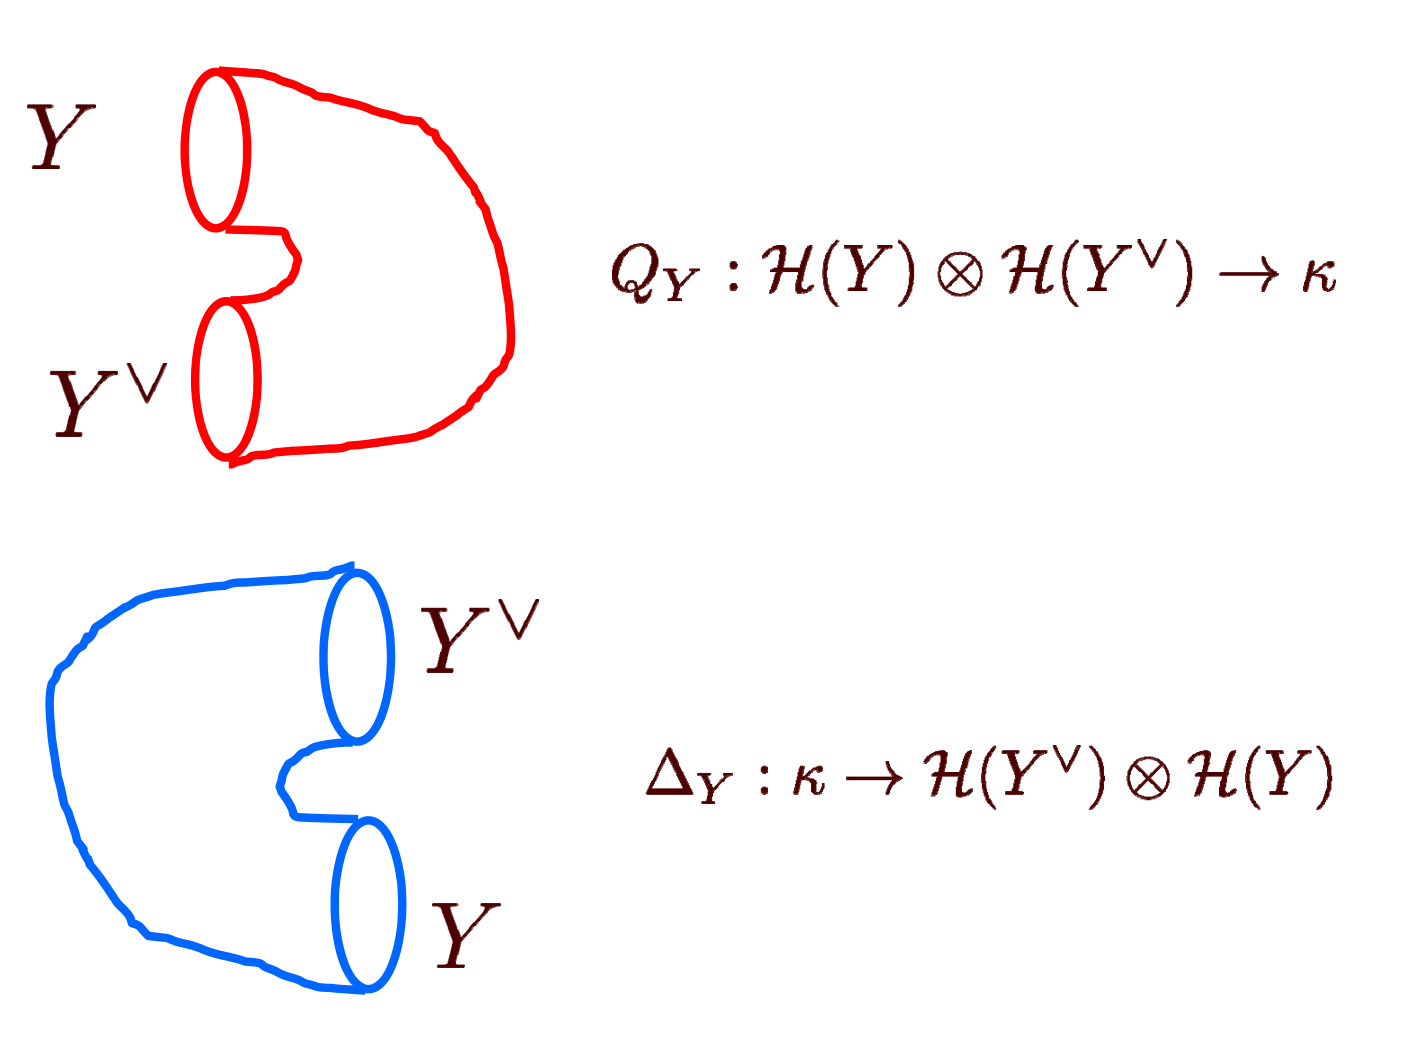
\includegraphics[width=0.50\textwidth]{figures/fig23.png}
  \caption{把柱弯折过来，以定义 $\Delta_Y$ 与 $Q_Y$。（原文 Fig.~23，第 151 页）}
  \label{fig:23}
\end{figure}

现在，让我们考虑有向配边范畴，于是 $Y$ 是有向的。以 $Y^\vee$ 记 $Y$ 取相反定向。配边 \eqref{eq:5.10} 与配边 $\emptyset\to Y^\vee\amalg Y$ 密切相关，后者定义一个映射
\begin{equation}
  \Delta_Y:\kappa\to\mathcal{H}(Y^\vee)\otimes\mathcal{H}(Y)
  \tag{5.11}
  \label{eq:5.11}
\end{equation}
它也与配边 $Y\amalg Y^\vee\to\emptyset$ 密切相关，后者定义一个二次型：
\begin{equation}
  Q_Y:\mathcal{H}(Y)\otimes\mathcal{H}(Y^\vee)\to\kappa
  \tag{5.12}
  \label{eq:5.12}
\end{equation}
现在把这些配边复合起来，我们就得到恒等映射，如图~\ref{fig:24} 所示。
% [原文此处作 "as in 24"（漏写了 Figure 一词），译文补出「图」字以便阅读]
于是由一些线性代数可知，$Q$ 是一个\emph{非退化}配对，从而我们有一个到线性对偶空间的同构：
\begin{equation*}
  \mathcal{H}(Y^\vee)\cong\mathcal{H}(Y)^\vee,
\end{equation*}

\begin{figure}[htbp]
  \centering
  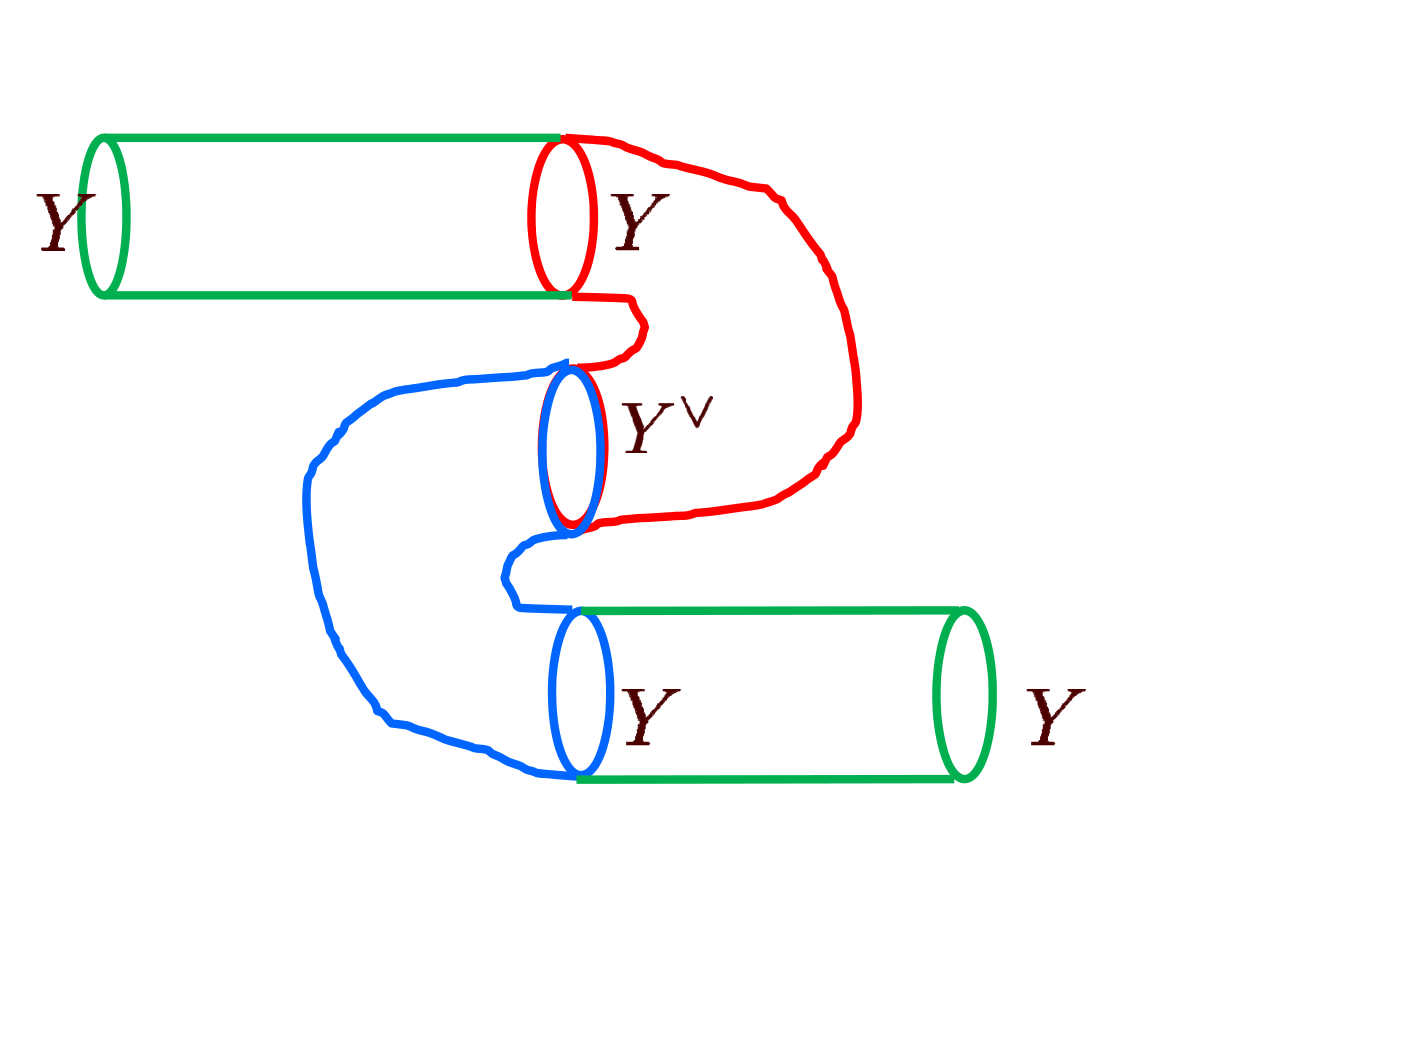
\includegraphics[width=0.50\textwidth]{figures/fig24.png}
  \caption{以某种方式复合 $\Delta\otimes1$ 与 $1\otimes Q$，使之给出 $P$。（原文 Fig.~24，第 152 页）}
  \label{fig:24}
\end{figure}

在这个同构下，$Q$ 恰好就是对偶配对。（左边 $Y^\vee$ 是 $Y$ 的定向反转，右边 $\mathcal{H}(Y)^\vee$ 是线性对偶空间。）
% [Tutor Note: 原文这句作 "(On the left $Y^\vee$ is $Y$ is the reversal of orientation...)"，多出一个 is，是排版笔误；译文按文意作「$Y^\vee$ 是 $Y$ 的定向反转」。同为易错点：这里的两个 $\vee$ 含义完全不同——$Y^\vee$ 是流形的定向反转，$\mathcal{H}(Y)^\vee$ 是向量空间的线性对偶，读 \eqref{eq:5.11}--\eqref{eq:5.12} 时必须分清]

为证明这一点，取 $\mathcal{H}(Y)$ 的一组基 $\{\phi_i\}$ 以及 $\mathcal{H}(Y^\vee)$ 的一组基 $\{\psi_a\}$。于是必须有
\begin{equation}
  \Delta_Y(1)=\sum_{i,a}\Delta^{ai}\psi_a\otimes\phi_i
  \tag{5.13}
  \label{eq:5.13}
\end{equation}
S-图表明
\begin{equation}
  \phi\to\sum_{i,a}\Delta^{ai}Q(\phi,\psi_a)\phi_i
  \tag{5.14}
  \label{eq:5.14}
\end{equation}
必须是恒等映射；于是取 $\phi=\phi_j$ 并定义 $Q_Y(\phi_j,\psi_a):=Q_{ja}$，就必须有
\begin{equation}
  \sum_a\Delta^{ai}Q_{ja}=\delta^i_{\ j}
  \tag{5.15}
  \label{eq:5.15}
\end{equation}
除此之外，我们还可以交换 $Y$ 与 $Y^\vee$ 的角色。计入 $\mathbb{Z}_2$-分次情形的符号（取齐次基），我们得到
\begin{equation}
  \sum_i\Delta^{ai}(-1)^{(|a|+|b|)|i|}Q_{ib}=\delta^a_{\ b}
  \tag{5.16}
  \label{eq:5.16}
\end{equation}
% [Tutor Note: \eqref{eq:5.13}--\eqref{eq:5.16} 的指标位置极易抄错：$\Delta^{ai}$ 的两个指标都写成上标（$\Delta_Y(1)$ 的展开系数），$Q_{ja}$、$Q_{ib}$ 的指标都在下标；$\delta^i_{\ j}$、$\delta^a_{\ b}$ 特意把下标错开一格，以免与 $\delta^i_j$ 混读。\eqref{eq:5.16} 中的符号 $(-1)^{(|a|+|b|)|i|}$ 是分次情形下的 Koszul 符号（$|a|$ 表示基向量 $\psi_a$ 的 $\mathbb{Z}_2$-次数）；在非分次极限下它退化为 $1$，\eqref{eq:5.16} 即回到 \eqref{eq:5.15}，核对时可据此作自洽性检查]
由此可知 $Q$ 可逆，故该配对是非退化的。这也就意味着存在上面所断言的同构 $\mathcal{H}(Y^\vee)\cong\mathcal{H}(Y)^\vee$。此外，选取一个同构使得 $Q_{i,a}=\delta_{i,a}$，现在用指标 $i$ 标记对偶基，并在该基下把记号 $\psi_i$ 改为 $\psi^i$，我们就简单地有
\begin{equation}
  \Delta_Y(1)=\sum_i\psi^i\otimes\phi_i
  \tag{5.17}
  \label{eq:5.17}
\end{equation}
现在，结果 \eqref{eq:5.17} 引出一个要点。若 $\mathcal{H}(Y)$ 是无穷维的，\eqref{eq:5.17} 是否收敛并不显然。事实上，即便 $\mathcal{H}(Y)$ 是赋范向量空间或 Hilbert 空间、从而向量无穷和的收敛确有定义，由于 $\phi_i$ 与 $\phi^i$ 是对偶基，只要 $\mathcal{H}(Y)$ 无穷维，这个和就不会收敛。\emph{因此，态空间 $\mathcal{H}(Y)$ 必须是有限维的！}
% [Tutor Note: 作者用 "It is not obvious" 略去了真正的论证：对偶基满足 $\phi^i(\phi_j)=\delta^i_{\ j}$，于是 $\sum_i\psi^i\otimes\phi_i$ 作用在任一态上给出 $\sum_i c_i\psi^i$，其系数全为 $1$；在无穷维情形这个和既不强收敛也不弱收敛（它是「对所有 $i$ 都取 $1$」这一非 $L^2$ 序列），故 \eqref{eq:5.17} 只能在某种分布意义/拓扑张量积下理解。这正是「Hilbert 空间必须有限维」的实质，也是下文所说「部分定义」的拓扑场论的由来；关于配边范畴中对象与态射的严格处理可查附录 K、L]

有许多有趣的「拓扑场论」例子，其中 $\mathcal{H}(Y)$ 明确是无穷维的。我们将在下文对此加以评论。

\begin{figure}[htbp]
  \centering
  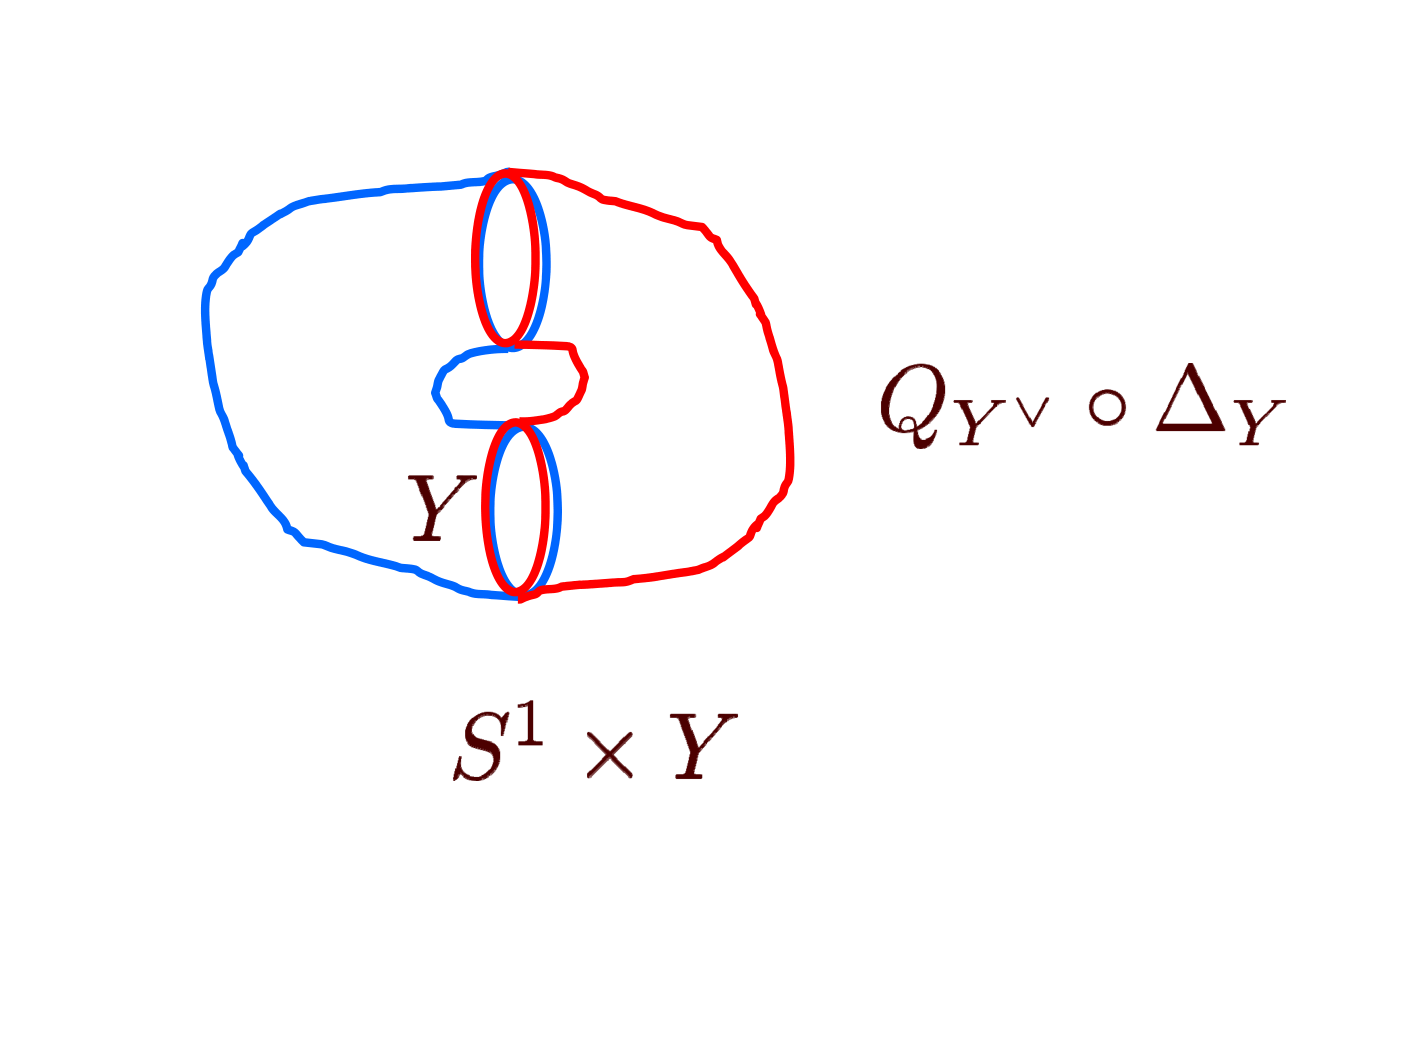
\includegraphics[width=0.45\textwidth]{figures/fig25.png}
  \caption{把 $Q_{Y^\vee}$ 与 $\Delta_Y$ 复合起来；在 $\mathbb{Z}_2$-分次情形它给出 $\mathcal{H}(Y)$ 的超维数，在非分次情形则给出 $\dim\mathcal{H}(Y)=Z(Y\times S^1)$。（原文 Fig.~25，第 153 页）}
  \label{fig:25}
\end{figure}

现在考虑图~\ref{fig:25} 中的图。一方面，这恰是配分函数 $Z(Y\times S^1)$。另一方面，线性映射 $\kappa\to\kappa$ 必须是复合 $Q_{Y^\vee}\Delta_Y$，或者等价地，$Q_Y\circ\Omega\circ\Delta_Y:\kappa\to\kappa$。由上面关于 $\Delta_Y(1)$ 的公式我们看到，$Z(Y\times S^1)$ 的值恰是维数 $\dim\mathcal{H}(Y)$，或者在 $\mathbb{Z}_2$-分次情形是超维数
\begin{equation}
  \operatorname{sdim}\mathcal{H}(Y)=\dim\mathcal{H}(Y)_0-\dim\mathcal{H}(Y)_1
  \tag{5.18}
  \label{eq:5.18}
\end{equation}

\textbf{评注}

\begin{enumerate}
  \item 注意若把范畴换成带 Riemann 结构的流形范畴，并在 $Y\times S^1$ 上取乘积 Riemann 结构，则
\begin{equation}
  Z(Y\times S^1)=\operatorname{Tr}e^{-\beta H}
  \tag{5.19}
  \label{eq:5.19}
\end{equation}
其中 $\beta$ 是圆的半径，$H$ 是 Hamilton 量。
% [Tutor Note: \eqref{eq:5.19} 与 \eqref{eq:5.18} 的对照是本节最易出错处：在 $\mathbb{Z}_2$-分次情形，能与 \eqref{eq:5.18} 相符的迹必须是超迹 $\operatorname{Tr}(-1)^F e^{-\beta H}$，而 \eqref{eq:5.19} 写的是普通迹——两者只在非分次情形一致。此外原文称 $\beta$ 为圆的半径；按 $Z=\operatorname{Tr}e^{-\beta H}$ 的标准推导，$\beta$ 实际是 $S^1$ 的周长（温度的倒数），若真的取半径为 $\beta$，指数上应出现 $2\pi\beta H$。两处均照原文转写，未作订正]
  \item 物理文献中有些重要的「拓扑场论」例子是违反这一条件的。一例是取非紧规范群的 Chern-Simons 理论。另一例是面积元为零的二维 Yang-Mills 理论。这些都是「部分定义」的拓扑场论：它们只在配边范畴中对象的一个子集上有定义。{\small\itshape ［原文标记：再说详细些。］}
% [原文待办标记（页边），原文 p.154：原文作 \ensuremath{\clubsuit}Say more. \ensuremath{\clubsuit}，作者自留的补充提示]
  \item 上面的 S-图论证指出了在对称幺半范畴中定义对偶对象（dual object）的路子。对偶对象 $x\in\operatorname{Obj}(C)$ 是指这样的对象：存在对象 $x^\vee\in\operatorname{Obj}(C)$ 以及态射 $\delta_x:1_C\to x\otimes x^\vee$ 与 $q_x:x^\vee\otimes x\to1_C$，使得
\begin{equation}
  x\xrightarrow{\iota_L(x)^{-1}}1_C\otimes x\xrightarrow{\delta_x\otimes1_x}x\otimes x^\vee\otimes x\xrightarrow{1_x\otimes q_x}x\otimes1_C\xrightarrow{\iota_R(x)}x
  \tag{5.20}
  \label{eq:5.20}
\end{equation}
并且（为简单起见，省略与张量单位相乘的同构）
\begin{equation}
  x^\vee\xrightarrow{1_{x^\vee}\otimes\delta_x}x^\vee\otimes x\otimes x^\vee\xrightarrow{q_x\otimes1_{x^\vee}}x^\vee
  \tag{5.21}
  \label{eq:5.21}
\end{equation}
都是恒等态射。
\end{enumerate}
% [Tutor Note: \eqref{eq:5.20}--\eqref{eq:5.21} 这两个复合等于恒等态射，就是张量范畴中的「蛇形（zig-zag）恒等式」，它们是把前面 S-图的拓扑事实转写成代数公理的结果。抄写时注意三处细节：单位同构记作 $\iota_L,\iota_R$（左、右单位同构）而非 $l,r$；$\delta_x$ 与 $q_x$ 的下标是对象 $x$ 而非流形 $Y$（与 \eqref{eq:5.11}--\eqref{eq:5.12} 的 $\Delta_Y,Q_Y$ 是同一构型的范畴化）；\eqref{eq:5.21} 中作者明言省略了与张量单位相乘的同构，故该链的两端只写到 $x^\vee$。术语取舍：「dual object」译作「对偶对象」、「dual pairing」译作「对偶配对」，「linear dual space」译作「线性对偶空间」，三者中文都用「对偶」以免与「自伴/共轭」混淆]

\begin{figure}[htbp]
  \centering
  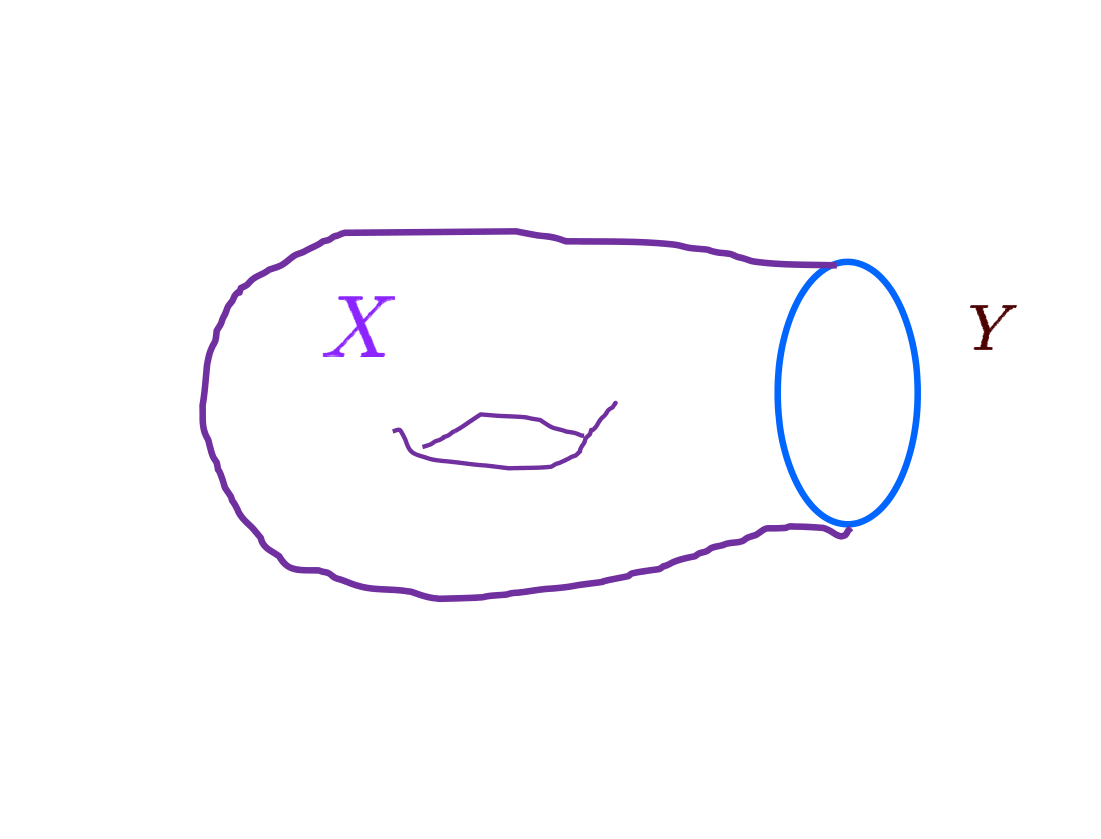
\includegraphics[width=0.50\textwidth]{figures/fig26.png}
  \caption{由从 $\emptyset$ 到 $Y$ 的一条配边所生成的一个态。（原文 Fig.~26，第 154 页）}
  \label{fig:26}
\end{figure}

\begin{figure}[htbp]
  \centering
  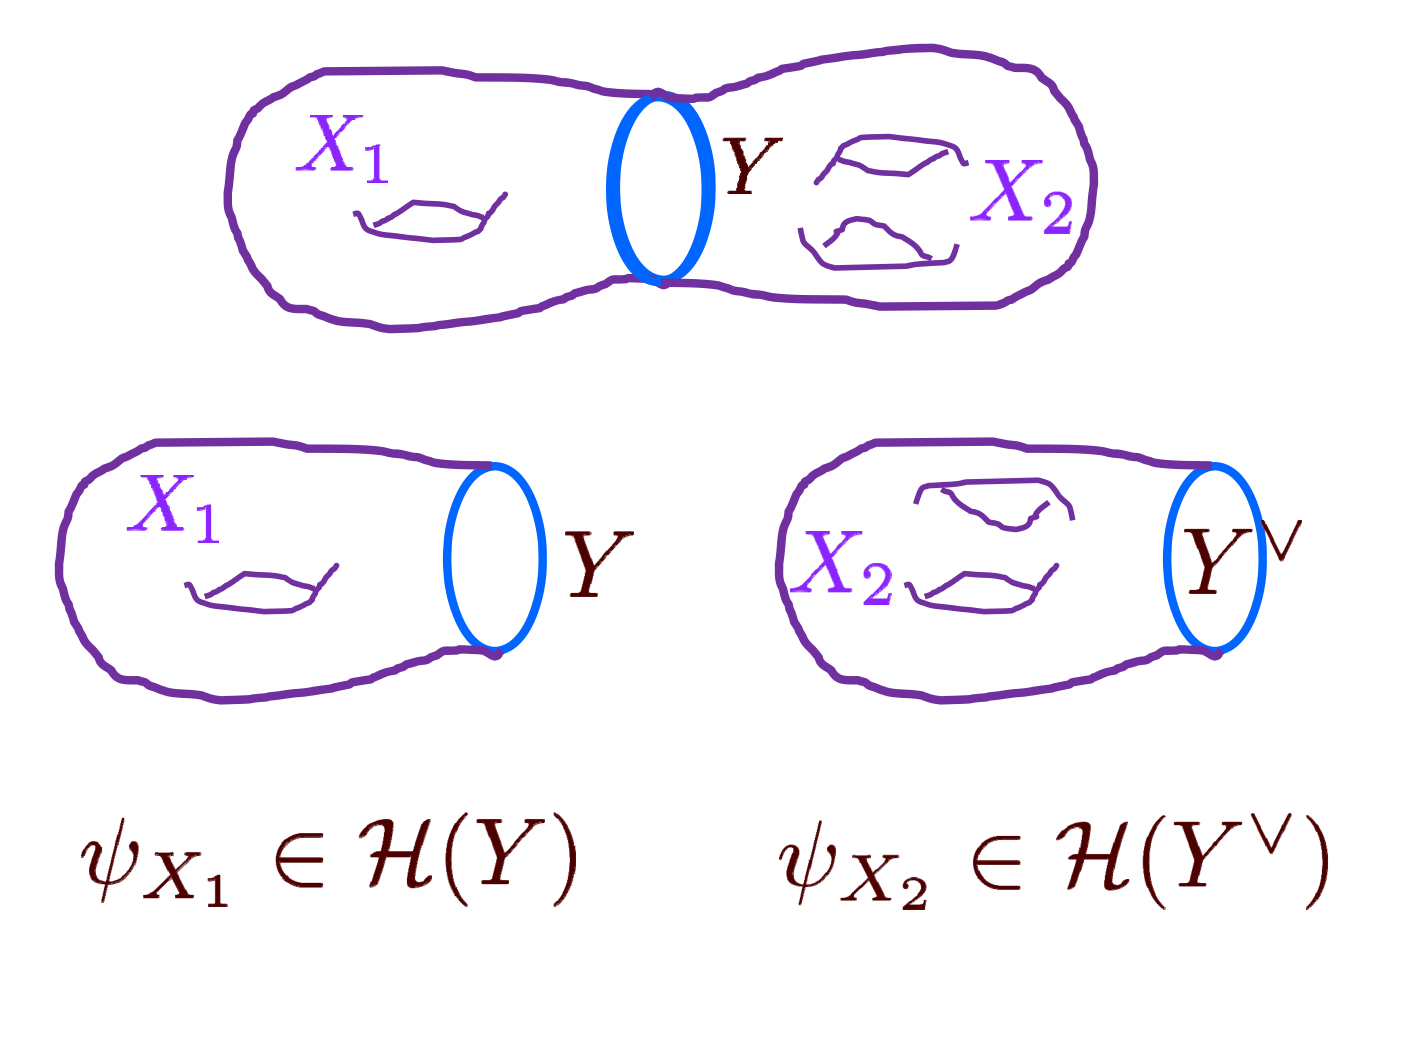
\includegraphics[width=0.50\textwidth]{figures/fig27.png}
  \caption{若闭流形 $X$ 沿一个余维一的子流形 $Y$ 切开，而 $Y$ 把 $X$ 分成两块 $X_1$ 与 $X_2$，则有两个相应的态 $\psi_{X_1}\in\mathcal{H}(Y)$ 与 $\psi_{X_2}\in\mathcal{H}(Y^\vee)$；配分函数 $Z(X)$ 的值可以看作这两个态用非退化配对 $Q_Y$ 所作的自然缩并。（原文 Fig.~27，第 155 页）}
  \label{fig:27}
\end{figure}

\medskip\noindent\textbf{练习}\quad\emph{映射柱与微分同胚群的特征标}

设 $f\in\operatorname{Diff}(Y)$，考虑映射柱 $M_f(Y)=([0,1]\times Y)/\!\sim$，其中我们把 $(0,y)$ 与 $(1,f(y))$ 等同起来。回忆 $\mathcal{H}(Y)$ 上有微分同胚群的表示 $\rho(f)$。

证明
\begin{equation}
  Z(M_f(Y))=\operatorname{Tr}_{\mathcal{H}(Y)}\rho(f)
  \tag{5.22}
  \label{eq:5.22}
\end{equation}
是微分同胚群的一个特征标。

事实上，$\rho(f)$ 只依赖于 $f$ 在映射类群（mapping class group）$\Gamma_Y$ 中的像：$\Gamma_Y$ 的定义如下——与恒等映射同痕（isotopic）的微分同胚构成全微分同胚群的一个正规子群 $\operatorname{Diff}_0(Y)$，而 $\Gamma_Y:=\operatorname{Diff}(Y)/\operatorname{Diff}_0(Y)$。{\small\itshape ［原文标记：详细解释 $\rho(f)$ 在 $f$ 的同痕下的独立性如何由公理推出。］}
% [原文待办标记（页边竖排），原文 p.155：原文作 \ensuremath{\clubsuit}Explain in detail how the independence of ρ(f) under isotopy of f follows from the axioms.\ensuremath{\clubsuit}，插在 "This is ... defined as follows" 之间]
% [Tutor Note: \eqref{eq:5.22} 是 \eqref{eq:5.18} 的「带扭转」版本：当 $f=Id$ 时 $M_f(Y)=Y\times S^1$，\eqref{eq:5.22} 退化为 $Z(Y\times S^1)=\operatorname{Tr}_{H(Y)}Id=\dim\mathcal{H}(Y)$，与 \eqref{eq:5.18} 一致（分次情形须改用超迹，参见 \eqref{eq:5.19} 的批注）。另外，作者在页边标记处想说的是：$\rho(f)$ 只依赖 $f$ 的同痕类，这一点的证明要用到「同痕可通过在 $[0,1]\times Y$ 上作微分同胚、把它在两端拉成恒等」这一事实；这正是把 \eqref{eq:5.22} 写成映射类群的特征标而非微分同胚群的特征标的依据]

\medskip\noindent\textbf{练习}\quad\emph{Hartle-Hawking 态与作为内积的配分函数}
% [原文标题误拼为 "Hartle-Hawking sates"，译文按 states 处理]

a.) 证明：任意配边 $X:\emptyset\to Y$ 都在空间 $\mathcal{H}(Y)$ 中定义一个\emph{态}。（见图~\ref{fig:26}。）拓扑场论的函子给出一个映射 $F(X):\kappa\to\mathcal{H}(Y)$，于是我们可以定义
\begin{equation}
  \psi_X:=F(X)(1)\in\mathcal{H}(Y)
  \tag{5.23}
  \label{eq:5.23}
\end{equation}
